\chapter{Background}
\label{chap:related_work}


This chapter presents the reasons why intrusion tolerance is needed, and then it describes the most relevant related works in the different intrusion tolerance areas.
It covers mainly the state-of-the-art of \gls{bft} replication, the techniques to rejuvenate replicas, and the benefits of using software diversity on distributed and replicated systems.
It also presents a few practical attempts to build systems that comprise these techniques.
Finally, it describes some of the works on vulnerability analysis and how such analysis can be used to improve classical intrusion-tolerant systems.


\section{The Need for Intrusion Tolerance}
The realistic way to provide security is to build mechanisms that protect potentially vulnerable systems from attackers.
This is particularly important when considering critical systems that attract highly motivated attackers. 
Here, the focus is on designing mechanisms to make systems safer and resilient despite their number of vulnerabilities and the attacker's power.
In the following, we make an overview of the different approaches that can be combined to deal with the challenge of providing security and dependability for critical systems.

\subsection{Vulnerability Prevention}
One of the primary techniques to stop attackers is to try to avoid that vulnerabilities persist in the code throughout the software development phases until it is used in production. 
One way to do that is to detect and remove vulnerabilities during the development and testing stages.
Here, we distinguish six different approaches that attempt to prevent software vulnerabilities. 

First, the most basic approach is manual analysis, typically developers (named testers) or automatic tools perform a set of tests that validate program inputs and outputs.
Often, in this type of analysis, the tester needs to check the results manually. 
The accuracy of the solution depends on how well the inputs cover all the behavior of the software and if the tester detects the output violations after (a description of this process is presented~\cite{Votipka:2018}).


Model checking is another approach, which abstracts the software code and formally verifies the program invariants.
However, the most common techniques typically over-simplify the protocols to make them formally verifiable or just use very particular version to verify~\cite{Klein:2009,Chen:2015,Nelson:2017}. 
Moreover, this process consumes much time, and it is expensive for most of the companies, which makes this method difficult to scale to complex systems~\cite{Giuffrida:2013}.
For example, an \gls{os} kernel was formally verified~\cite{Klein:2009}, but contrary to the Linux kernel that has more than 20 million lines of code\footnote{Source: https://www.linuxcounter.net/statistics/kernel on 2nd July 2018} this only has 10k lines of code.


One way to find pieces of code that could harm the correctness of the software is to resort to static vulnerability analyzers.
This type of analysis is typically limited as it looks for small parts of the code that alone may not cause major alarm.
Additionally, it is exhaustive and depends on the availability of the source code.
On the contrary, in the software's reliability area, there are significant advances in automatic and efficient error detection~\cite{Xu:2016}.
A particular technique used in security that tackles both coverage and code complexity is taint analysis.
In this technique, any program variable that can be modified by a user is seen as a vulnerability trigger. 
Then, when it is accessed, it becomes tainted for further inspection.
The main limitations of taint analysis are that vulnerabilities are detected only for the execution paths that have been explored by the tester, and it is limited to call/return functions being challenging to cover shared memory or global variables~\cite{Yamaguchi:2015}.


Another conventional solution to explore software bugs is fuzzing.
Fuzzing is a dynamic technique, as it runs against executing software, and its success in finding vulnerabilities or bugs results from a good set of input test cases.
These can be built manually and tuned for a particular application, or randomly generated, for the latter they are likely to fail on triggering more complex vulnerabilities.
The main limitation of fuzzing is the time it takes to perform, as it tries multiple execution paths during the test~\cite{Gan:2018}.


There are also solutions that combine some of the previously described techniques like taint analysis and fuzzing.
For example, concolic testing is a technique that performs symbolic execution along with a concrete execution path~\cite{Kim:2017}. 
Therefore, it is more accurate than fuzzing, but it tends to succumb to path explosion.
Some of these techniques can be combined to take the best of some of the approaches described before~\cite{Stephens:2016}.


Finally, some works proposed workarounds that intended to minimize the window of vulnerability between vulnerability disclosure and the patch release.
Typically, these solutions have two phases: first, the detection phase where they look for vulnerabilities in the source code, and a second one, where they instrument the code with the vulnerability workaround.
Although they may have good coverage of the vulnerabilities, there are a few caveats on applying such solution.
For example, some workarounds may crash the application upon the vulnerability activation, or they may disable the main functions that clients use in the software~\cite{Huang:2016}, i.e., compromising the availability. 


Although these techniques are steps towards more robust software, they all have limitations on coverage, either they fail to cover the whole code surface, or they fail to detect more complex and unknown vulnerabilities.
Moreover, these techniques are especially useful to use before the vulnerable system is in production.


\subsection{Fault Detection and Removal}
Most of the previously described techniques work offline and are not complete. 
Therefore, unknown vulnerabilities may arise when the system is already online, allowing the system to be compromised.
Then, we need a more complex approach to cope with the existence of vulnerabilities that can be exploited.
The detection and removal approach works by detecting intrusions at runtime and then triggering a recovery mechanism to clear the resulting effects. 

Since some attacks employ a combination of different vulnerabilities, which isolated would be harmless, it is hard to detect them when the system is in production. 
This approach presents three problems: 
First, there are no perfect intrusion detectors, and therefore, stealth attacks may remain active for long intervals; 
Second, the service can experience some periods of unavailability while the service is recovering; 
Finally, recovering a system might clean its faults, but the system remains vulnerable.
Therefore, depending on the flow, it could be easy for an attacker to repeat the same procedure to compromise the system every time it recovers.


\subsection{Fault Tolerance and Masking}
The previously described approaches assume that vulnerability removal can be achieved or that is possible to detect all the attacks.
However, these assumptions are unrealistic, and it is not advisable to trust the security and dependability of a sole approach, as it creates a single point-of-failure. 
Thus, once the system becomes compromised the whole infrastructure becomes exposed to more attacks. 

The established way to build a system with tolerance and masking properties is to base its implementation on a group of replicas, which execute equal commands in the same order. 
Primary-backup replication (i.e., $1 + 1$ replicas), would suffice if only crash faults are considered. 
If one of the replicas stops executing, the other can replace it and deliver the service correctly.
However, if arbitrary faults are considered, this form of primary-backup replication is not enough because compromised replicas could return arbitrary outputs to the clients, impeding the correct answer to be delivered.

\gls{smr}~\cite{Lamport:1984} is an approach that has been employed to ensure fault tolerance~\cite{Schneider:1990} of fundamental services in modern internet-scale infrastructures (e.g.,~\cite{Hunt:2010,Calder:2011,Corbett:2013}).
\gls{smr} is achieved in distributed systems that run an agreement protocol that guarantees that all the replica nodes (i) start from the same state, (ii) process an equal sequence of messages, and (iii) execute the same state transitions. 
These properties guarantee that a service runs in a similar manner in all replicas, and therefore, they all produce the same outputs.
However, \gls{smr} must resort to intrusion tolerance techniques~\cite{Verissimo:2003} to address malicious (or sometimes called Byzantine) faults.

Intrusion tolerance was first proposed by Fraga and Powell~\cite{Fraga:1985} as a solution to address faults without compromising the security of a system. 
More formally, we adopt the following intrusion tolerance definition: 

\begin{defn}
\emph{``A replicated intrusion-tolerant system is a replicated system in which a malicious adversary needs to compromise more than $f$ out-of $n$ components in less than $T$ time units to make it fail.''}~\cite{Bessani:2011}
\label{def:def2}
\end{defn}

It is necessary to employ \gls{bft} \gls{smr}, a particular case of \gls{smr}, to build a system capable of operating correctly even in the presence of some compromised replicas.
Since no single replica can be trusted completely, the correctness of the system comes from the majority of correct nodes.
For example, to tolerate a single fault (i.e., $f=1$) the system must have four replicas, where $n \geq 3f+1$~\cite{Castro:2002}.
Although \gls{bft} protocols provide safety to a bound of $f$ faulty nodes, with sufficient time (i.e., greater than $T$), an adversary could eventually compromise $f+1$ nodes.
Then, additional mechanisms are needed to clean the faulty state, for example, from time to time the nodes are recovered~\cite{Castro:2002}.
However, if a recovered node remains vulnerable to the same attack, the time to compromise $f+1$ replicas becomes smaller as the attacker already knows how to exploit the existing vulnerabilities.
For this reason, several authors have built their systems assuming that nodes fail independently due to some mechanism that provides failure independence (e.g.,~\cite{Castro:2002,Bessani:2008,Veronese:2013,Sousa:2010}).
For instance, to increase the time $T$ that takes to compromise $f+1$, one could employ periodic recoveries to reset the replicas' faulty state. 
Moreover, to avoid reintroducing replicas with the same vulnerabilities in the system, the recovery should change the replica's code somehow.
Finally, the recovery procedure needs to managed carefully because otherwise, the decisions that are made with no criteria could lead to a decrease of $T$.
If bad decisions are made, e.g., deploying $f+1$ replicas with shared weaknesses, an attacker can replicate the same attack on the sufficient number of replicas to compromise the whole system (i.e., $f+1$).
Otherwise, an attacker needs to create $f+1$ different exploits and apply them to $f+1$ replicas before $T$. 
In the following sections, we present and describe several works on specific areas of intrusion tolerance, covering the various issues that we have just mentioned.


\section{Byzantine Fault Tolerance}

Castro and Liskov’s \textsc{Pbft}~\cite{Castro:1999} was the first practical \gls{bft} replicated system, and it was initially proposed as a solution to handle faults of both accidental and malicious nature.
The correctness of a \gls{bft} service arises from the existence of a quorum of correct nodes capable of reaching consensus on the (total) order of messages to be delivered to the replicas.
\textsc{Pbft} implements a \gls{smr} protocol that guarantees safety for up to $\lfloor\frac{n-1}{3}\rfloor$ faulty replicas out of a total of $n$. 
To tolerate a single replica failure, this sort of system typically must have four replicas. 
This property holds even in asynchronous systems such as the internet. 

\textsc{Pbft} implemented a \gls{smr}, therefore, it guarantees that each correct replica executes the same commands, in the same order, and then it produces the same output. 
In Figure~\ref{fig:bft}, we present an overview of the \textsc{Pbft} protocol that can be summarized as follows:
A client \emph{(c)} sends a message to all the replicas \emph{(R1-R4)} requesting the execution of some service (or operation).
Then, the leader replica has to assign a sequence number to the request and multicasts a \emph{propose} message to the other replicas. 
If the replicas agree with the leader, they send a \emph{write} message to each other. 
At this phase of the protocol, every correct replica agrees on the ordering of the messages.  
Next, every replica multicasts an \emph{accept} message. 
When correct replicas receive the \emph{accept} messages from a quorum, then they execute the request deterministically. 
In the end, it replies to the client, which waits for $f+1$ equal responses to guarantee that the correct response is delivered.

Every replica shares a key with each other and with clients. 
These keys are used to authenticate messages with a \gls{mac}. 
The messages that are multicast by the clients are authenticated with a vector of \glspl{mac}. 
Then, each replica verifies its own \gls{mac}.
The authors validated this \gls{bft} library implementing a Byzantine fault-tolerant file system. 
The results show that when the workload increases the throughput and latency is nearly the same as a non-replicated system. 

\begin{figure}[h]
\begin{center}
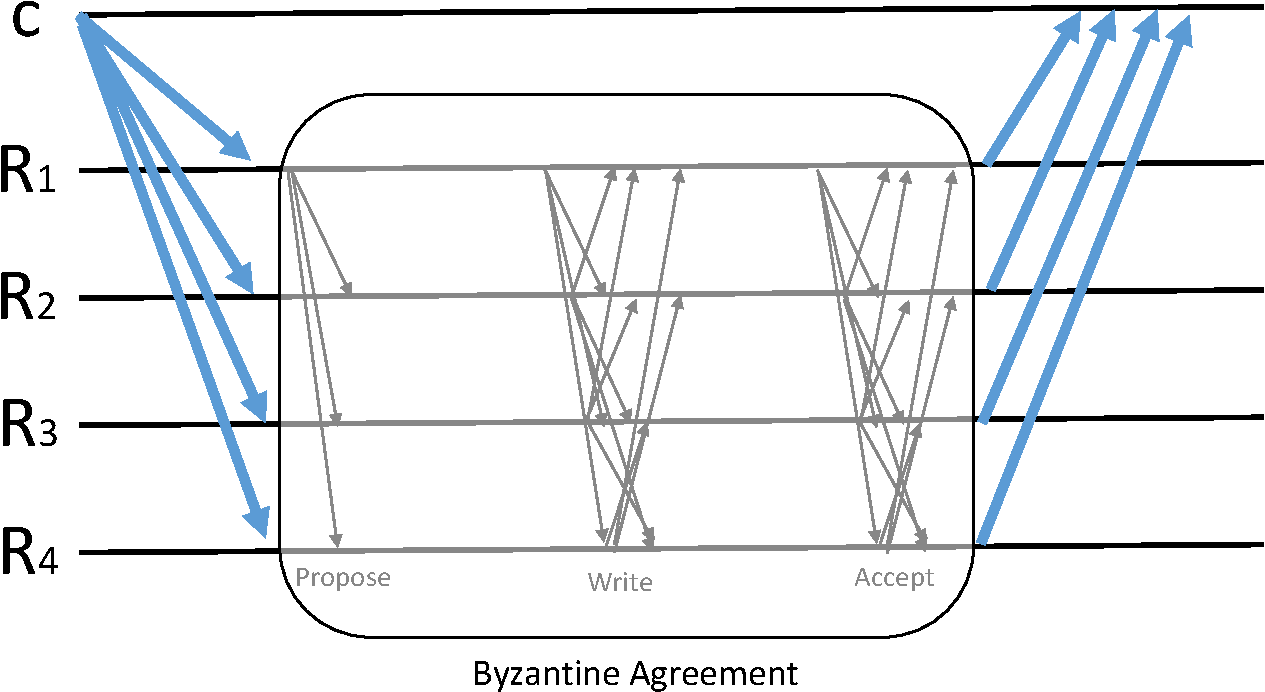
\includegraphics[width=.7\columnwidth]{images/images/bft.pdf}
\caption{Byzantine Fault Tolerance protocol overview, where \emph{C} represents a client of a replicated service enumerated by replicas \emph{Ri}.}
\label{fig:bft}
\end{center}
\end{figure}

\textsc{Pbft} good performance encouraged the use of \gls{bft} in common systems, and to develop optimizations to improve \gls{bft} protocols. 
Since the \textsc{Pbft} proposal, many solutions have been dedicated to improve \gls{bft} protocols in a different manner. 
Table~\ref{tab:bft} gives an overview of a few of them.


\begin{table}[h]
\begin{center}
{\footnotesize
\begin{tabular}{ p{2.5cm}  p{10.0cm}  }\hline
\textsc{Zyzzyva}~\cite{Kotla:2010}  & Introduced speculation to avoid the expensive three-phase commit before processing the requests. This might introduce some inconsistency in the state of the replicas when speculation fails and needs the help from the client to fix the problem. \\ \hline            
\textsc{Aardvark}~\cite{Clement:2009b} & Shifted the paradigm to a new design. This design improved the performance under faulty scenarios trading some performance on the normal case. The decision was to design a system that prefers safety over performance on gracious executions. Some counter-intuitive decisions on the architecture favored the overall execution on both gracious and fault scenarios. \\ \hline
\textsc{Upright}~\cite{Clement:2009} & It provided a straightforward way to support crash fault-tolerant systems, without having to run as many replicas. It combined the protocol of \textsc{Zyzzyva} and the mechanisms of \textsc{Aardvark}. It did not require cryptographic signatures as it uses a \glspl{mac} matrix instead. \\ \hline    
\textsc{MinBFT}~\cite{Veronese:2013}  & Reduced the number $n$ from $3f+1$ to $2f+1$ by leveraging on trusted components. These components are deemed as trusted as it hardware is simple and thus verified. Additionally, this solution reduced one communication step compared to other BFT protocols. \\ \hline
\textsc{BFT-SMaRt}~\cite{Bessani:2014} & It was developed to be a modular and multicore-aware. It also supports replica reconfiguration, as it allows that replicas leave and join the replica group. In this process, the joined replicas received the state from the correct replicas in order to be up to date. It also has a flexible programming interface that simplifies its use. \\ \hline
\textsc{COP}~\cite{Behl:2015} & It is one of the most recent BFT implementations, having reached 2.4 million operations per second. This was achieved mostly due to BFT architecture changes, like the creation of \emph{consensus instances} which are assigned to a client or a group of clients. These (separated) \emph{consensus instances} are executed in parallel increasing the throughput of the system.\\  \hline  
\end{tabular}
}
\caption{Brief overview of the most relevant BFT works.}

\label{tab:bft}
\end{center}
\end{table}




\paragraph{Summary.} 

In this thesis, we propose a control plane for \gls{bft} systems.
The aim is to guarantee that replicas execute correctly while tolerating malicious failures in a subset of them.
The implementation of such \gls{bft} protocol is a complex task, namely if it supports mechanisms for state transfer and reconfiguration while ensuring good performance.
Therefore, we prefer to rely on existent libraries than to build a new one.
Nevertheless, for some contributions (see Chapter~\ref{chap:sieveq}), we needed to perform some modifications on the chosen library.



\section{Replica Rejuvenation}
Software rejuvenation was proposed in the 90's~\cite{Huang:1993,Huang:1995} as a proactive approach to prevent component performance degradation and failures due to software aging. 
This solution was implemented using three components: a watchdog process (\texttt{watchd}), a checkpoint library (\texttt{libft}) and a replication mechanism (\texttt{REPL}). 
A primary component executes the application and also runs the \texttt{watchd} to monitor the application crashes and hangs. 
The backup component keeps its application inactive and observes the primary node in order to be able to substitute it. 
Additionally, there is a routine (provided by \texttt{libft}) that periodically makes checkpoints and logs messages. 
These checkpoints are replicated with \texttt{REPL} in the backup node. 
When the primary node crashes or hangs, it is restarted, and if needed the backup takes his place on the execution.


Some years later, proactive recovery was also adopted on \gls{bft} replicated systems by Castro and Liskov~\cite{Castro:2002}.
In order to support long-running services, the aim is to rejuvenate replicas periodically to eliminate the effects that an attacker could have caused on a faulty node. 
This mechanism allows that the system remains correct as long as the adversary controls up to $f$ replicas before a recovery.
Moreover, \textsc{Pbft} introduced additional mechanisms to guarantee that \gls{smr} properties are maintained even with recoveries.
In particular, a \emph{state transfer} protocol, which allows that recovered replicas fetch a correct and up to date state from the other (correct) replicas.
Additional assumptions were needed to guarantee the \textsc{Pbft} liveness and safety during the recoveries: 
(i) each replica contains a trusted chip to store its private key, and it can sign and decrypt messages without revealing the key; 
(ii) the replicas' public keys are stored in a read-only memory, which needs physical access to be modified; 
and (iii) a watchdog timer is used to avoid human interaction to restart replicas. 
The watchdog hands the execution to the recovery monitor, which cannot be interrupted.

An alternative way to \gls{smr} to implement \gls{bft} systems is to resort to quorum systems.
Zhou~\etal{}~\cite{Zhou:2002} presented \textsc{Coca}, a fault-tolerant online certification authority to be deployed both in a local area network and on the internet.
It also employed proactive recovery to rejuvenate replicas' state including the capacity to refresh the private keys of the replicas.
The adoption of quorum systems does not require timing assumptions and, contrary to \textsc{Pbft}, \textsc{Coca} did not rely on trusted components.
However, these options may compromise the safety (i.e., $f$ faulty nodes in-between recoveries) of the systems under asynchronous environments as it was shown by Sousa~\etal{}~\cite{Sousa:2007}. 
Sousa~\etal{} demonstrated the need for hybrid-systems that require some level of synchrony to guarantee safety and liveness of proactive recovery systems.


Virtualization was later identified, by Reiser and Kapitza~\cite{Reiser:2007} and Distler~\etal{}~\cite{Distler:2008}, as a useful mechanism to implement proactive recovery.
They proposed an architecture, named \textsc{Vm-Fit}, that was divided into two parts: an untrusted domain and a trusted domain.
The intrusion-tolerant replicated system executes in the untrusted domain where replicas run in a separate \gls{vm}. 
\textsc{Vm-Fit} executes in a trusted domain, i.e., in the \gls{vmm}. 
Virtualization provides isolation between the untrusted and the trusted domains. 
Therefore, the trusted domain can trigger recoveries in a synchronous manner. 
Moreover, virtualization reduces downtime of the service during the recovery and makes the state transfer between replicas more efficient. 
The authors implemented this system using the Xen hypervisor.
The trusted domain is placed in the hypervisor \texttt{Dom0}, and the replicas run in the untrusted \glspl{vm}, \texttt{DomUs}.

Dealing with the presence of faults that cannot be detected was the drive for the work of Sousa~\etal{}~\cite{Sousa:2010}.
The authors suggested improvements to recovery mechanisms by introducing the \gls{prrw}. 
It accelerated the rejuvenation process by detecting the faulty replicas behavior and forcing them to recover without sacrificing periodic rejuvenations. 
This type of technique can only be implemented with synchrony assumptions as the rejuvenations are time triggered~\cite{Sousa:2005}. 
To address this need, the authors proposed a hybrid system model: the payload was an any-synchrony subsystem where the replicas execute, and the wormhole was a synchronous subsystem. 
The authors implemented this approach using the Xen hypervisor as the wormhole. 
Zhao~\etal{}~\cite{Zhao:2012} improved \gls{prrw} with an algorithm to schedule the rejuvenations that are triggered by monitoring the network and CPU/memory performance.


\paragraph{Summary.} 
\gls{bft} replication with proactive recovery represents one of the cornerstones of intrusion tolerance. 
Proactive recovery allows the system to reduce the replicas' vulnerability window by cleaning the faulty states, impeding the attacker to be successful at compromising more than $f$ replicas simultaneously. 
Nevertheless, \gls{bft} replication with proactive recovery guarantees the system's correctness while replicas recover before $f+1$ replicas become faulty. 
All works on \emph{safe} proactive recovery require the use of a trusted local component on each replica to trigger the periodic recoveries~\cite{Castro:2002,Sousa:2010,Roeder:2010,Platania:2014,Distler:2011}.
Some of these works used hardware timers while others resorted to virtualization to separate the execution domains. 
In our proposal, we adopt an architecture inspired on~\cite{Distler:2008} and~\cite{Sousa:2010}. 
However, our solution implements a different (from~\cite{Sousa:2010}) algorithm to trigger recoveries.
More importantly, most of these solutions assumed that replicas fail independently without addressing that issue, which is a topic central to our research
The following section reviews diversity as a way to overcome failure independence difficulties. 




\section{Diversity}
In all works presented before, the correctness of the \gls{bft} system is ensured under the assumption that replicas fail independently.
Therefore, it is assumed implicitly (or explicitly) that there is some mechanism that creates different vulnerable surfaces, which would increase substantially the effort to exploit each replica.
One practical way to achieve this is to build diverse replicas.

Diversity can be implemented in different manners~\cite{Deswarte:1998,Larsen:2015}, which may differ in the mean and on the amount of diversity generated, but the goal is the same: to create different attack surfaces (details in the survey~\cite{Baudry:2015}).\side{Conference on Computer Security, Dependability, and Assurance: From Needs to Solutions 1998, Trans. Sec. Priv 2015, ACM Computer Surveys 2015}
In particular, it decreases the chances of finding a vulnerability that compromises $f+1$ replicas at the same time~\cite{Castro:2002}.
In other words, diversity would contribute to avoiding common vulnerabilities among replicas. 
We present three different approaches to attain diversity: 
(i) N-version programming consists of designing and/or implementing  different versions from the same specification; 
(ii) Automatic diversity by implementing different memory organization schemes and compiling distinct binary executables (from the same source); 
and (iii) \gls{ots} diversity comprises the use of different products with similar functionality, but taking advantage of the various implementations that are already available.


\subsection{N-version Programming}
The first work on diversity was published in 1975 by Randell~\etal{}~\cite{Randell:1975}. 
They introduced the idea of using different software design (i.e., implementations) as a way to achieve reliable software. 
The idea is to deploy additional and different replicas along the primary replica, and once the replicas have a mismatch result, a spare replica follows up as primary.


Chen and Avizienis~\cite{Avizienis:1977,Chen:1978} defined the notion of N-version programming with the goal of achieving software reliability in redundant systems.
The principle was to resort to $N$ teams that would develop $N$ versions of the same software specification that would be semantically equivalent.
Then, the N-version programs would execute and compare the outputs.
If the outputs were equivalent, then the result was accepted.
These works opened research avenues in the area of security and reliability.
In any case, Knight and Leveson~\cite{Knight:1986} made an empirical study that concludes that N-version must be employed with particular care, as it for itself may not provide increased reliability guarantees. 

\subsection{Automatic Diversity}  
The idea of having to $N$ different teams to develop $N$ software versions was not attractive from several perspectives (including the cost), and soon appeared automatic approaches for introducing diversity.
Forrest~\etal{}~\cite{Forrest:1997} suggested randomized program transformations to introduce application diversity.
They have made modifications to \texttt{gcc}, the GNU C Compiler, in such a way that at compiling time random padding is inserted into each stack frame. 
The diverse versions are generated therefore during the source code compilation, and these works aim to make the intruder’s work more difficult when exploiting buffer overflow vulnerabilities.
More recently, a few other works propose the usage of diversity-based compilers to build different executables~\cite{Platania:2014,Roeder:2010,King:2016,Koo:2018}.


Hosek and Cadar~\cite{Hosek:2015} proposed \textsc{Varan}, an N-version Execution framework.
\textsc{Varan} is composed of a leader replica and its followers that share a memory ring where they execute in parallel.
These components are launched by a coordinator that orchestrates and setups the execution environment.
Each follower runs a binary that has system calls rewritten differently, and this optimization plays a significant performance improvement when compared with other solutions that rewrite the whole program.
The implementation of the memory ring is also a major improvement as it allows concurrent access by multiple producers and consumers.
Nevertheless, the results show that some system calls when executed in \textsc{Varan} can introduce overheads (e.g., of 36\% for \texttt{close} and 240\% for \texttt{open}) when compared with a native setup.
The authors also scale out the number of followers, which, as expected, increases the overhead as they are added. 
Although \textsc{Varan} was purposed for reliability, some principles could be adopted in the security domain after solving some challenges, namely the use of the same address space that would allow return-oriented programming attacks.

\textsc{Bunshin} by Xu~\etal{} works as classic N-version systems, the N variants receive the input execute it and then a voter checks for divergences in the output.
However, \textsc{Bunshin} does not create real N-versions, in fact, it splits the program into parts, and each part (of each variant) executes some security check. 
In this way, they can reduce the overheads of typical N-variant solutions as the code is very practically the same while creating different checks that should capture faulty behavior.
Most of the overhead introduced is due to the variants synchronization before the output voting.
Nevertheless, the security of the systems holds on the assumption that an attacker cannot easily overpass the sanity checks.
Moreover, it is even more challenging to overpass them in all variants, which make sense for more straightforward attacks.


A different approach based on memory address obfuscation (i.e., \gls{aslr}) was proposed by Bhatkar~\etal{}~\cite{Bhatkar:2003}.
Their solution transformed object files and executables at the link- and load-time, without kernel or compiler modifications. 
The goal is to ensure that an attack that compromises one target will not succeed on the other targets. 
Each time the program is executed its virtual addresses and data are randomized, and therefore the attacker needs to find new ways to exploit memory errors like buffer overflows. 
However, recent works have shown that solutions like \gls{aslr} are still vulnerable to attacks~\cite{Bittau:2014,Jang:2016,Snow:2013,vanderVeen:2017}.

As it was observed in a survey, by Larsen~\etal{}~\cite{Larsen:2015}, it is quite difficult to measure the efficacy of automatic techniques.
For example, entropy analysis may consider two versions of a binary as high entropy but, they could be equally vulnerable to a specific attack.
Another way to evaluate these solutions is to test them against real attacks, but this would raise coverage issues.
Moreover, to evaluate automatic diversity is time-consuming and it tends to over-generalize.


\subsection{Off-the-shelf Diversity}
The previous approaches generate diversity before software’s distribution. 
On the contrary, \gls{ots} diversity does not need pre-distribution of diverse mechanisms. 
It relies on the existence of different software components that are ready to be used.
There are plenty of products that provide the same functionality and were developed by distinct vendors. 
In other words, \gls{cots} diversity is like opportunistic N-version programming.


\paragraph{Studies.}
There are a few works that study the diversity of \gls{cots} as a way to achieve failure independence.
Han~\etal{}~\cite{Han:2009} made a systematic analysis of the effectiveness of using \gls{ots} diversity to improve the system's security.
First, the authors tried to find if there were software substitutes to provide the same functionality. 
Then, they determined if the \gls{ots} software shared the same vulnerabilities and if so, if the same vulnerability could be exploited with the same attack. 
In this study, they analyzed more than 6k vulnerabilities from \gls{nvd}. 
The results showed that 98.5$\%$ of the vulnerable software had substitutes. 
Moreover, the majority of them did not have the same vulnerabilities or could not be compromised with the same exploit code. 
It is not expected that a single exploit works in different \glspl{os} because each one has a different memory scheme and file system. 
Even between releases from the same \gls{os}, the low-level functions sometimes change across the versions. 
The study also concluded that 22.5$\%$ of the vulnerabilities were present in multiple software components. 
However, only 7.1$\%$ from those vulnerabilities were present in software that offers the same service. 
The study findings are a good sign that diversity can improve a system’s dependability.

Gashi~\etal{}~\cite{Gashi:2007} made an experimental evaluation of the benefits of adopting different \gls{sql} databases.
The authors analyzed bug reports of four database servers (PostgreSQL, Interbase, Oracle, and Microsoft \gls{sql} Server) and determined which products were affected by each bug reported. 
They have found few cases of a single bug compromising more than one server. 
In fact, there were no coincident failures in more than two of the servers.
The conclusion was that \gls{ots} database servers’ diversity is an effective mean to improve the system's reliability. 
However, the authors recognize the need for \gls{sql} translators, to increase the interoperability between servers in the replicated scenario.

In the same line of the Gashi~\etal{}, Garcia~\etal{}~\cite{Garcia:2012} studied the vulnerabilities shared among \gls{ots} \glspl{os}.
Similar to \cite{Han:2009}, this study was carried out taking as input the vulnerability feeds from \gls{nvd}. 
However, this work was only focused on \glspl{os}, and the dataset comprised 11-years of vulnerability reports. 
Their goal was to find to what extent different \glspl{os} had common vulnerabilities. 
To do that, they analyzed 2270 vulnerabilities entries manually and classified them into different categories. 
Then, the authors defined three types of servers: (i) a server that contained most the packages/applications available (Fat server); (ii) a server that did not contain unnecessary applications to a particular service (Thin server); and (iii) a thin server but with physically controlled access (Isolated thin server). 
They assumed that the third setting was the most advisable for critical systems because additional care is taken to install and setup its software. 
For each configuration, they compared all the common vulnerabilities in pairs of \glspl{os}. 
As expected, in the Isolated thin server, the number of common vulnerabilities was considerably less than in the other configurations. 
There was only one vulnerability that was shared among six \glspl{os}, two that were shared among five \glspl{os}, and 130 that are shared between two \glspl{os}. 
They went further in the study and looked for common vulnerabilities in different versions of the same \gls{os}. 
Even if few \glspl{os} are employed, it is possible to achieve vulnerability independence just with different versions.
The authors have found evidence that suggests that using OS diversity in a replicated system can improve its dependability. 



\paragraph{Network diversity.}
Diversity assignment was also used as a solution to increase the network's resiliency (in particular its connectivity).
Newell~\etal{}~\cite{Newell:2015} presented their solution as a Diversity Assignment Problem, that although it is an NP-hard to solve, the authors showed that for medium-size random networks graphs it was feasible to find solutions within an acceptable time.
They used mixed-integer programming for medium-sized networks and for larger networks they proposed a fast greedy approach.
For the first one, it was possible to achieve optimality, and for the latter an approximation of the optimal.
One of the results showed that random diversity assignment is far worse than a criteria assignment (as the one they proposed).
Their results showed improvements of diversity on the connectivity (i.e., resiliency).
However, their models did not use realistic data, as the authors assumed that the expectancy values for the probability of node compromise were known and independent for each replica.


In the same line, Zhang~\etal{}~\cite{Zhang:2016} proposed a metric to evaluate the resilience of private networks.
The idea was to define what is the least attacking effort to compromise some critical assets of the network (i.e., the work is focused on distributed yet not replicated systems).
Therefore, they measured the weakest path to the target that compromises the main asset. 
The authors proposed three metrics which were evaluated in a simulated environment.
None of these metrics used vulnerability data to correlate the existence of common weaknesses, and on the contrary, the metrics used data about the topology, services installed, etc.
The authors made a simulated evaluation of generated graph networks and evaluated their metric against these graphs. 
The results show that increasing the diversity on the nodes reduced the worm propagation on the network.
 

\paragraph{Summary.}
We presented three different techniques that support diversity as a fault tolerance mechanism. 
Classical N-version programming is the most costly since it needs different developers and additional programs to verify if the automatic translations work. 
On the contrary, \gls{ots} and some automatic diversity (like randomization) are almost for free. 
The first one can be obtained from components that are ready to be used, and the second one is automatic and already supported in most \glspl{os}. 
Diversity still has some gaps that must be addressed to make it a useful building block of intrusion tolerance. 
For example, how does one measure diversity as a contribution to increasing failure independence?


\section{Practical Systems with Diversity}
Despite the existence of several studies on vulnerabilities, a few works implemented diversity to some level in their systems.
Totel~\etal{}~\cite{Totel:2005} proposed an \gls{ids} based on design diversity.
The authors described an architecture that uses a set of replicated \gls{cots} servers, a proxy, and an \gls{ids}. 
The proxy is responsible for forwarding the requests from the client to every \gls{cots} server. 
When the servers reply, the proxy sends the responses to the \gls{ids} to be analyzed. 
The IDS compares the responses from the \gls{cots} servers, and if it detects some differences, an alarm is raised. 
Next, the proxy votes the responses and replies to the clients. 
The authors developed an algorithm to detect intrusions and tested their solutions against Snort~\cite{snort} and WebStat~\cite{Vigna:2003}. 
The results showed that using a diverse-\gls{cots} service (e.g., HTTP) allows the \gls{ids} to deliver fewer alarms without missing the intrusions.

Bairavasundaram and Sundararaman~\cite{Bairavasundaram:2009} implemented \textsc{EnvyFS}, a file system that uses N-version file systems implementations to guarantee the reliability of stored data.
Their solution is able to tolerate file system mistakes (e.g., crash and integrity errors). 
To keep the system simple, the authors used a virtual file system layer that abstract the specific file systems underneath, therefore some challenges arise from the different implementations details.
Another challenge was to avoid the need for multiple storages as it uses N-variants of file systems. 
They solved this issue by resorting to only one storage layer and the different file systems in between. 
Each file system executes the operations, and then a voter collects the majority of outputs to the storage layer.
The results showed that \textsc{EnvyFS} is able to improve the reliability by leveraging on multiple file systems.
However, \textsc{EnvyFS} performance pays a performance penalty due to waiting for a majority of file systems responses. 
In most of the times, it took the sum of the time of the three file systems used.

Diversity has also been adopted to build a malware detector. 
Xu and Kim~\cite{Xu:2017} introduced \textsc{PlatPal} that analyzes the behavioral discrepancies of malicious document files on different platforms (e.g.,Windows or Macintosh).
\textsc{PlatPal} loads a file in both systems and monitors the execution traces or crashes. 
In the end, both systems compare the outputs, and an attack is signaled if divergences are observed.
The authors focused on a particular application, the Adobe Acrobat Reader.
It reads and displays pdf files, and both \glspl{os} have the application available.
Therefore, besides the internal discrepancies, the correct executions should be very similar.
There are some limitations, namely, it failed to detect attacks that needed some human interaction.
Although \textsc{PlatPal} was proposed to detect malicious payloads on files, it vouched (indirectly) for diversity as it showed that an attacker needed to deploy multiple payloads to compromise a system with the same attack (for the majority of the malware samples used).

\paragraph{Diversity on BFT.}
A few \gls{bft} works already adopted practical diversity mechanisms. 
One of the first proposals was \textsc{Base}~\cite{Castro:2003}, an extension of \textsc{Pbft}~\cite{Castro:1999} that explored opportunistic \gls{ots} diversity in \gls{bft} replication.
The system provided an abstraction layer for running diverse service codebases on top of the \textsc{Pbft} library.
The key issue addressed by \textsc{Base} was how to deal with different representations of the replica's state, allowing a replica that recovers from a failure to rebuild its state from other replicas. 
\textsc{Base} was evaluated considering four different \glspl{os} and their native \gls{nfs} implementations: Linux, OpenBSD, Solaris, and FreeBSD.
The results showed that performance varied significantly when diversity was considered.
Nevertheless, \textsc{Base} did not address the problem of selecting replicas nor the reconfiguration of the replica group.

Roeder and Schneider~\cite{Roeder:2010} proposed a solution that combined an automatic diversity with rejuvenations, they called it \gls{po}.
The idea was to change the application and library code periodically, while preserving the original semantics by employing program transformations, i.e., system call obfuscation reordering, memory randomization, and functions return checks (through an IBM \texttt{gcc} patch that inserts and checks a random value after the functions return).
Each replica generated its own obfuscated executable from a read-only device containing the ``master code'' based, on time-triggered epochs that a controller initiates in a secure way through a trusted component.
All obfuscation mechanisms were implemented and evaluated on OpenBSD 4.0, and their results showed that \gls{po} adds little extra overhead to the non-\gls{po} execution.

A similar approach by Platania~\etal{}~\cite{Platania:2014} adopted a compiler-based diversity for the \textsc{Prime} \gls{bft} library~\cite{Amir:2011} using the MultiCompiler tool~\cite{Homescu:2013}.
This compiler was used to create diverse binaries from the same source code through randomization and padding techniques.
The authors also proposed a theoretical rejuvenation model that received as input: the probability of a replica being correct over a year ($c$); the number of rejuvenations per day across the whole system ($r$); the number of replicas ($n$); and the system's lifetime. 
Although operators can control only $r$ and $n$, the authors suggested (but did not show how) that $c$ would be estimated using \gls{osint} from the internet (CERT alerts, bug reports, and other historical data).
The authors implemented their solution in two settings, including a virtualized environment provided by the Xen Hypervisor.
In this setting, each replica executed in a Linux \gls{vm}, the recovery watchdog runs in a trusted domain of the same machine, and the proactive-recovery controller runs in another physical machine. In Chapter~\ref{chap:lazarus_implementation} we present an architecture that evolves from this one.


\paragraph{Summary.} 
Diversity is becoming one of the building blocks of intrusion tolerance, alongside with \gls{bft} and rejuvenations. 
We presented few works that already used in some manner diversity in intrusion-tolerant settings. 
Although we do not discard the possibility of employing other diversity techniques, such as randomization, we are more interested in \gls{cots} diversity.
\gls{cots} diversity allows us to use data that is freely available, to estimate a risk value that measures how vulnerable is each component. 

Previous works are still limited to that extent, e.g., there are none or few concerns on how to create diversity to avoid common failures. 
They implement diversity assuming complete fault independence, but that is unrealistic. 
For example, different \gls{ots} \glspl{os} can share the same weaknesses due to some shared libraries or kernel code. 
There is a need to understand how diversity can be efficiently employed in a replicated system to make failure independence sound. 
Moreover, further work is still necessary to create automatic mechanisms that abstract diversity management for the administrators.



\section{Vulnerability Analysis}
In another line of research, a few works were devoted to analyzing vulnerabilities life-cycle and evolution.
Massacci and Nguyen~\cite{Massacci:2010} analyzed several data sources that provide data about vulnerabilities, exploits, and patches.
The authors mentioned some limitations on the data sources.
For example, that is difficult to integrate the different sources due to naming and ID differences across them.
In the following, we present several studies on vulnerability data that is used to measure and manage the security of computer systems.


The different stages of vulnerability life-cycle were described by Jumratjaroenvanit and Teng-Amnuay~\cite{Jumratjaroenvanit:2008}.
The authors' goal was to understand how the various life-cycle dates can be useful to estimate the probability of an attack. 
The methodology was to collect and analyze data from public data sources on the discovery-, disclosure-, exploit-date and exploit-, patch-availability. 
They used this information to define five life cycle types: (i) \gls{zda}, which typically is done by a black-hat, and is characterized by equal dates of disclosure and exploit; (ii) \gls{pzda}, which is a \gls{zda} but with a patch already available, but not applied; 
(iii) \gls{ppzda} is a \gls{pzda} but does not matter if the patch is available or not; 
(iv) \gls{poa} is a zero-day vulnerability. 
The most influential variables were the programs that were scrutinized by the tester with access to the source code, and the programs that were analyzed with some static analysis tool. 
The results showed that language safety was the less influential factor. 
The study also demonstrated was that two weeks of work were enough to have a 50\% chance of finding a zero-day vulnerability. 
Sometimes 53 hours were enough to find one vulnerability with more than 95\% of probability.


Frei~\etal{}~\cite{Frei:2010} made a quantitative analysis of 27k vulnerabilities disclosed in the last decade.
The authors proposed a model that explains the leading players in a vulnerability lifecycle.
All the dates associated with the vulnerability lifecycle were described in detail before the analysis.
A few public vulnerability databases (e.g., \gls{nvd} and \gls{osvdb}) were used to collect the different data attributes.
The results showed that the number of patches increased after the vulnerability's disclosure.  
One interesting result was the \emph{the gap of insecurity} measurement, where the patch availability was compared against the exploit availability. 
The data showed that exploits are always ahead of patches.
In some cases, after 30 days of the disclosure, the exploits outnumbered the number of patches by 90\%.


A study conducted, by Shahzad~\etal{}~\cite{Shahzad:2012}, analyzed data between 1988 to 2011 from three sources: \gls{nvd}, \gls{osvdb}, and the dataset from Frei and colleagues~\cite{Frei:2006}.
They collected vulnerabilities that affected popular applications like Internet Explorer, Firefox, and Chrome, and popular \glspl{os} such as Windows, Mac OS X, Solaris and several Linux distributions. 
It was found that 2006 was the peak year for vulnerability disclosures, and since then there was a decrease even with more software products available. 
However, the complexity of the disclosed vulnerabilities has increased, based on the score of the \gls{cvss}. 
From their dataset, 2.8\% vulnerabilities have an exploit released before the public disclosure. 
More dramatic is the percentage of exploits that are released on the day of the vulnerability disclosure, which was in the order of 88.2\%. 
It was observed that 9.7\% of the vulnerabilities had exploits released after their disclosure.
Microsoft and Apple had more exploits before the vulnerability disclosure than the other software providers. 
This may primarily be because hackers find it more rewarding to exploit these products due to their broader market capitalization.
To what concerns patching, the authors argue that 10\% of the vulnerabilities had a patch before their disclosure, and 62\% had a patch on its disclosure day. 
There was a considerable number of vulnerabilities that were disclosed only after a patch was made available, more precisely 28\%. 
Another conclusion was that it is easier to exploit opensource code vulnerabilities than in closed-source – this conclusion may seem obvious, but no one had shown it previously with statistical tests.

Zero-day vulnerabilities between 2008-2011 were part of a systematic study by Bilge and Dumitras~\cite{Bilge:2012}.
The main dataset comes from the \gls{wine} (developed by Symantec), which samples and aggregates data from several hosts running Symantec products (e.g., Norton Antivirus).
The \gls{wine} data was correlated with \gls{osvdb} and Symantec's Threat Explorer for attack/exploit information, allowing the measurement of the duration of zero-day attacks.
They conclude that the average attack lasts ten months. 
Moreover, they found that another threat had exploited two years before Stuxnet some of the vulnerabilities exploited in this attack.
One of the main conclusions was that the disclosure of zero-day vulnerabilities increases the risk, up to five orders of magnitude, of users being attacked.
Therefore, the vendors would be responsible for prioritizing the disclosure of such vulnerabilities and preparing a patch as soon as possible. 


Holm~\cite{Holm:2014} made an analysis of malware alarms to verify if there is a statistical distribution to model the number of intrusions or the time to compromise a computer system.
The author collected information from different software configurations from 2009 to 2012 from an IT enterprise.
During this period, the enterprise had a total of 697 \glspl{os} and versions, which were considered in the evaluation.
Each computer was equipped with anti-malware software, and when malware is detected, it sent some logging data to a central database.
The results showed that the Pareto distribution is the one that best fits to model the time of the first compromise.
Another result was that the more the system is intruded, the more vulnerable it becomes. 
The author presented a few hypotheses for this result, for example, once a system was broken it can no longer be trusted. 
Another and more plausible hypothesis is that security awareness only increased in temporarily as a result of the intrusion, and then it is again neglected.
Automatic attacks caused most of the malware considered in this study.
This is probably due to the type of enterprise. 
Conclusions may change if malware come due to targeted attacks as they require a different strategy to penetrate the system.

Contrary to the most common approaches that attempt to measure the vulnerability state of a system, Wang~\etal{}~\cite{Wang:2014} proposed a different approach to assess this.
The authors explored how many zero-day vulnerabilities were required to compromise a network. 
As they did not consider replication, but instead a ``chained'' architecture, the use of diversity enhances the security of the overall network, but each service in the network is not dependable.
One of the limitations of this approach was that it considered all zero-day vulnerabilities equally likely to occur.
Moreover, the metric's calculation is complex, and no evaluation is provided to hint to the reader on how long can it take to calculate.


Poolsappasit~\etal{}~\cite{Poolsappasit:2012} described a security risk assessment method that incorporated the cause-effect relationships of the network states and the likelihood of exploiting such relationships.
To do that, they measured the organizations' security risk using \gls{cvss} metric.
The authors implemented a tool that generates a map of the network as a Bayesian attack graph.
Then, it collects data with a vulnerability scanner, and it fetches the vulnerability exposures for each vulnerability.
The result is helpful for system administrators that can have an overview of the network weaknesses and associate a cost to the assets in a way that countermeasures can be taken to avoid such weaknesses.
The countermeasures are indicated by the system administrator that will link them to the attributes model.
Then, the administrator assigns the damage costs to every attribute.
Finally, a genetic algorithm evolves the network for states where the cost of losing assets (i.e., being compromised) is minimal. 
Their empirical results show the costs of being compromised can be minimized by assessing the security of the system and applying the most cost-efficient countermeasures.
Nevertheless, and besides the manual setup that the system administrator needs to perform, a time evaluation is missing on how the system reacts when an attack is detected.


The patch deployment process of ten popular client applications was analyzed over a five-year period by Nappa~\etal{}~\cite{Nappa:2015}.
In some cases, where applications shared libraries, the patching process took a different time from the same vulnerable shared code.
The authors have found that there was a strong correlation between the vulnerability disclosure and the start patching process among vendors.
It occurred within seven days for 77\% of the studied vulnerabilities.
A \emph{survival analysis} (inspired in medicine and biology to measure the mortality rates associated with diseases) was performed to measure the probability of a vulnerable host remains vulnerable beyond a specific time.
The vulnerability ``dies'' once a patch is installed or a non-vulnerable software is installed.
The experimental results showed that real-world WINE exploits still compromised 50\% of the vulnerable hosts (after vulnerabilities disclosure). 
The median percentage of hosts that have been patched before the exploit was released was at most 14\%.
Together with the number of shared vulnerable code with different patching delays, these values motivate attackers to re-used already known exploits or to create patched-based exploits~\cite{Brumley:2008}.
The authors also showed evidence to support the natural intuition that silent or automatic updates reduce the survivability of vulnerabilities. 
They also performed an analysis on three different user profiles, which showed that security analysts were more careful on patching software than software developers or regular users.


Machine-learning techniques were employed, by Bozorgi~\etal{}~\cite{Bozorgi:2010}, to classify vulnerabilities and predict future exploits.
Their results showed that their trained classifiers outperform current exploitability measures like \gls{cvss} exploitability subscore.
They have built a dataset based on two public databases, the Mitre' \gls{cve} (which is a subpart of \gls{nvd}) and the \gls{osvdb}.
The bag-of-words machine learning technique was utilized to extract the textual attributes that were more relevant to analyze.
They also resorted to \gls{svm} to train the model and conduct offline and online experiments.
In the offline setting, which they trained and evaluated data in a static fashion, they achieved an accuracy of 90\% of correct predictions.
In the online setting, the results showed that after a small period the model stabilized and reduced the overall error by 14\%.
Here, they were able to make predictions up to two days before the exploit was released with an accuracy of 75-80\%.
The main result, for the interest of this thesis, was the comparison between their model and the \gls{cvss} as an indicator of how a vulnerability was likely to be exploited.
The \gls{cvss} assigned high scores to vulnerabilities that did not become exploited. 


An in-depth analysis of four security databases, \gls{nvd}, Exploit-DB, SYM, and EKITS conducted by Allodi and Massacci~\cite{Allodi:2014}, \emph{break down} the \gls{cvss} on its several attributes.
For example, the exploitability subscore \emph{resembled more a constant than a variable}, thus not having a real impact on the \gls{cvss} overall score.
They used a randomized case-control study, which is applied to different study domains.
It was used to assess the effectiveness of treatment over a sample of subjects.
In this study, they measured how \gls{cvss} influences the \emph{risk factor} of the study cases.
A result that is worthy of note was that fixing vulnerabilities based on their \gls{cvss} was statistically equivalent to picking a random vulnerability to fix from the security relevance standpoint.
On the contrary, the authors suggest that it was more critical to fix vulnerabilities that appear in the black market of vulnerabilities (this was re-evaluated in a recent study by the same authors~\cite{Allodi:2017}).
The results indicated that the inclusion of black market information as a \emph{risk factor} could increase the risk reduction up to 80\%.
However, the authors also pointed out that using the EKITS data source may be a threat to the validity of the study, as it is unstructured data and therefore it requires manual analysis.



In the different and unusual data sources, Sabottke~\etal{}~\cite{Sabottke:2015} presented a study with Twitter data (e.g., specific words, the number of retweets, replies, and information about the users posting these messages) to find information about exploits. 
A quantitative and qualitative exploration was carried out over the vulnerability-related information disseminated on Twitter.
A Twitter-based exploit detector was developed to provide an adequate response in a such short time frame. 
This allows the security community to foresee the exploit activity before the information reaches the \emph{de facto} disclosure data sources, like \gls{nvd} and ExploitDB.
However, to complement and strengthen their information results, the paper also used sources like \gls{nvd}, \gls{osvdb}, Exploit-DB, Microsoft Security Advisories and Symantec WINE. 
Real-world exploits were distinguished from the proof-of-concept exploits, as the latter are by-products of the disclosure process. 
The real-world exploits typically are not known until a critical zero-day attack occurs. 
The authors used \gls{svm} to classify exploits in the social media and tested their robustness to attacks, i.e., if a powerful attack could manipulate the information on Twitter with false accounts and false data. 
The results showed that with their proposal there was a reasonable level of confidence about the predictions. 
For example, the \gls{svm} classifier set to a precision of 25\% could detect the Heartbleed exploits within 10 minutes of their first appearance on Twitter. 
They also showed that organizations like \gls{nvd} overestimate the severity of some vulnerabilities (with \gls{cvss}) that never become in fact exploited.


Gorbenko~\etal{}~\cite{Gorbenko:2017} resorted to the \gls{cve} and \gls{nvd} databases to study vulnerability life-cycles of different \glspl{os}.
The authors made a particular effort to analyze the relationship between vulnerability discovery and fix, more precisely the time vendors took to patch the vulnerable software.
Moreover, they also studied common vulnerabilities among different \glspl{os}.
The results show that between 2012 and 2016 most of \glspl{os} were patched for every vulnerability that was disclosed in that period (the only exception was Ubuntu Server 12.04).
Another interesting result was related to \emph{forever-day vulnerability} (i.e., vulnerabilities that are publicly disclosed but not yet patched). 
They showed that, for the analyzed period, Ubuntu never had a single day free from vulnerabilities, and Windows and Red Hat had only 12 and 10, respectively.
However, the most important results were the implications of \gls{cvss} on the \emph{days-of-gray-risk} (i.e., the number of days it takes for a vendor to release a patch). 
It was observed that there was no obvious implication on the level of \gls{cvss} severity and the time it took for a vendor to develop a patch.


Other works, not focused on replicated systems dependability, worked on malware prediction. 
In particular, \textsc{RiskTeller}~\cite{Bilge:2017}, proposed by Bilge~\etal{}, predicts the risk of a system becoming infected by malware.
In this work, the authors conducted a study that accounted for 600k machines belonging to 18 enterprises.
They collected the log data from all machines together with external data (e.g., from \gls{nvd}).
They defined a dataset with 89 features, such as patching behavior, temporal patterns, application categories, and past threat history.
\textsc{RiskTeller} was evaluated by using machine learning models to learn and classify the labeled software of each machine.
The results show that it can make predictions on the risk of a system being attacked with an accuracy of 96\%. 


\paragraph{Summary.} 
We presented several works that carried out the risk assessment in a way to prevent exploits or to take action upon vulnerability detection. 
This is the last building block that intrusion tolerance is missing. 
There is a lot of relevant free information available to address the security and dependability of software. 
In a replicated context this information is even more relevant. 
First, to react upon vulnerability/exploit disclosures, and second to select what configurations are less vulnerable to common weaknesses. 
We want to explore the free available data to improve the dependability and security of intrusion-tolerant systems, by ensuring the assumption of failure independence with evidence supported by relevant and sound information.
Additionally, some of the works proposed solutions to enhance the reliability and security of networks. 
In this thesis, we are concerned with the security and dependability of replicated systems. 
Hence, we are focused on assuring that no more than $f$ replicas become compromised.


\section{Management of Vulnerable Systems}
In the previous sections, we presented approaches to support the recovery and diversity of replicas, several of which in \gls{bft} replicated systems.
In this section, we focus on some works that already combine, in a very limited way, the idea of diversity and rejuvenations.
We review a few more recent works that introduce the idea of risk management (see~\cite{Yuan:2014} for a complete survey).


Reynolds~\etal{}~\cite{Reynolds:2002} presented the \textsc{Hacqit} fault-tolerant architecture.
It was build to assure fault tolerance by resorting on backup replicas on separate LANs and allowing only authorized clients through \gls{vpn}.
Moreover, it employed redundancy and diversity to detect and mask errors in the system components.
The same input is sent to identical nodes, and if the output is different, then some node is considered faulty. 
Thus it is possible to vote outputs, and the majority is considered as correct.
Moreover, it used a forensic agent that analyzed the logs of failed nodes to prevent bad requests in the future.
Finally, it implemented a recovery mechanism that was triggered by the native security auditing of Windows NT/2000.
Unfortunately, no experimental evaluation was presented.
Nevertheless, \textsc{Hacqit} was one of the first systems to promote all these mechanisms together.


Wang~\etal{}~\cite{Wang:2003} proposed an architecture, named \textsc{Sitar}, that aims to build intrusion-tolerant systems with diversity and dynamic reconfigurations.
\textsc{Sitar} defends a set of potentially vulnerable \gls{cots} servers. 
The system was protected by an intrusion-tolerant multilayer architecture that used redundancy and security protocols to guarantee that all nodes correctly agreed on the decisions.
It is composed of three main components: the proxy servers, the acceptor monitors, and the ballot monitors.
The proxies receive the requests and audit them based on the current threat level, and then they propagate the messages to the \gls{cots} servers. 
On the way back, the acceptance monitors validate the response and run an agreement protocol to select a final output from the \gls{cots} servers.
There was also an adaptive reconfiguration module that monitors the other modules, by receiving heartbeats and intrusion triggers to take action on removing compromised modules and starting new ones.
No results on diversity were shown.


The same type of solution was applied on cluster deployments.
Arsenault~\etal{}~\cite{Arsenault:2007} presented \gls{scit} a centralized architecture which goal was to recover the elements of a cluster without harming the availability of the overall service.
Recovering the cluster's nodes allows for resetting the state and avoiding huge windows of vulnerability.
Nevertheless, the \gls{scit} service itself can be harmed. 
Therefore, the authors leveraged on trusted hardware to offer additional guarantees to the system, namely predictable and continuous operation regardless of the presence of attacks.


Junqueira~\etal{}~\cite{Junqueira:2005} proposed \emph{informed replication}, as an approach to design distributed systems that can survive catastrophes.
It focused on the diversity of the components to avoid common pathogens that could compromise the entire system.
A new system model was adopted to map different attributes of a node. 
These attributes represented characteristics that should be distinct on each node to avoid common failures.
While modeling the system, some biases were introduced.
For instance, the authors considered that two different services that used the same port were vulnerable to the same vulnerability, or that the same service running with two different ports were not vulnerable.
A heuristic was proposed to build configurations in linear time.
The goal was to distribute the \glspl{os} and applications in different configurations, in such a way that minimized the number of common attributes that could compromise the configuration.
Two metrics were utilized to select \glspl{os} and applications, one selected them by pick random-uniformly both, and the other chosen them based on their popularity.
The results showed that their solution mitigated the number of pathogens that could compromise an entire configuration as its attributes were selected in order to maximize their difference.
The heuristic guaranteed 99\% chances of data survival on an attack of single- and double-exploit pathogens, while needing only three and five copies respectively.


More focused on reliability, Zhai~\etal{}~\cite{Zhai:2014} proposed a system that looks for failure independence on the cloud.
The system collected and audited data from the system components to evaluate their independence by identifying potential correlated failures.
Then, the different configuration dependencies were analyzed and ranked in risk groups as a way to see how the different dependencies made the system fail.
The main limitation of this work was that it depended on the will of cloud providers to share private data to be analyzed by external agents.
The authors evaluated the efficacy of their solution on finding the minimal risk groups (with fewer dependencies) on sampling data to make faster decisions while losing some accuracy.
The work's main focus was the reliability of cloud systems, thus no evaluation was done on vulnerabilities of such systems.

Seondong~\etal{}~\cite{Seondong:2017} described a system that used data from \gls{nvd} to select the best configuration of diverse \glspl{os} and web servers.
The algorithm minimized the \gls{cvss} of shared vulnerabilities among the various software components.
Although their experiments explored different configurations of software stacks, the decisions were based on the \gls{cvss}.
All the experiments were done in a simulator (i.e., CSIM 20) which made it difficult to understand the real performance of the solution.
Moreover, the resilience of the system was evaluated against \gls{dos} attacks that affect particular vulnerabilities in the software.
Depending on the type of the \gls{dos}, it can cause a performance decrease without exploiting any vulnerability.
This, however, does not shed light on the ability of the system to prevent $f+1$ replicas from being compromised.
In any case, this is the work that most resembles one of the main contributions of this thesis. 
However, it suffers some limitations that we will address in Chapter~\ref{chap:lazarus_design}.


\paragraph{Moving Target Defenses.} 
An emerging area, called \gls{mtd}, re-defines some of the already existing solutions with the goal of achieving a continuous change of the attack surfaces. 
\gls{mtd} employs techniques like \gls{vm} migration, different types of diversity, etc.
Some authors have made an effort to formalize this sub-area of intrusion tolerance~\cite{Zhuang:2014}.

Okhravi~\etal{}~\cite{Okhravi:2014} presented \textsc{Talent}, a framework for live migration of critical infrastructures across heterogeneous platforms.
The idea was to create a moving target that made advanced targeted attacks harder to succeed. 
\textsc{Talent} implemented \gls{os}-level virtualization with containers, which allowed the system to migrate the \gls{os} between machines periodically or upon detection of malicious activity. 
The virtualization was implemented with \texttt{OpenVZ} and \texttt{LXC} for Linux, \texttt{Virtuozzo} for Windows, and \texttt{Jail} for FreeBSD. 
The network was also virtualized, more precisely, a second layer of virtualization was used to migrate the IP address from one container to another. 
Even an established \texttt{ssh} session was preserved during the migration. 
Additionally, the state of the application also had to be migrated by employing a checkpointing technique. 
When all the programs were checkpointed, the state was saved and then was migrated by mirroring the file system. 
The file system synchronization took 98.7\% of the migration time. 
The authors decided to focus on optimizing the file system synchronization. 
In the optimized version, the file system synchronized in periodic intervals by sending the differences to the destination. 
Therefore, the migration was made seamless to the application. 
\textsc{Talent} also had a sort of risk assessment, called operation assessment, which monitored and adjusted the diverse components using vulnerability information. 
However, there were almost no details on how the risk was measured and on how to adapt to the threats efficiently.


\gls{mtd} was classified, Hong and Kim~\cite{Hong:2015}, into three categories, shuffle, diversity and redundancy, and assessed the effectiveness of each one.
The three solutions were integrated in \textsc{Harm} and it was evaluated how each technique could improve the security of distributed systems.
The solution was built on top of \glspl{vm}, as each \gls{vm} was able to host a few \glspl{os} in it.
Then, the evaluation scenarios considered three hosts running with two to three \glspl{vm} inside.
The three techniques were evaluated separately, and only two \glspl{os} were considered in the diversity evaluation.
In the considered scenarios, deploying random diversity did not improve the risk level of the system. 
For example, in one each host ideally had at least one \gls{vm} with a diverse \gls{os}.
On the other hand, having diverse \gls{os} across host decreased the connectivity, in case of some \gls{os} became compromised.
However, these sort of results was not surprising as only two \glspl{os} were considered.
On the contrary, with more \glspl{os} the system would maintain the level of connectivity while assuring the dependability of the hosts.
 

\paragraph{Summary.}
We presented a few control systems that manage nodes that are potentially vulnerable and exploitable.
Some of the works presented in other sections already combined a few of these mechanisms (e.g., Sousa~\etal{}~\cite{Sousa:2010} introduce reactive recovery upon detection of faulty behavior). 
However, only a few have implemented or discussed the real implications of using diversity (with the exceptions like BASE~\cite{Castro:2003} that implemented \gls{ots} diversity and assessed its performance overhead).


\section{Final Remarks}
In this chapter, we described the most relevant works that are related to this thesis.
We have made background revision of the intrusion tolerance area, and then we described the different topics that support intrusion-tolerant systems.
Our main contributions are on the management of \gls{bft} systems, in particular, how to create diverse replicas that effectively are independent and when the replicas need to be recovered. 
Although we could adopt solutions from artificial diversity, we are more interested in employing \gls{ots} diversity.
\gls{ots} diversity allow us to use data to make decisions on which diverse options work better together.
Such decisions would take action as rejuvenation triggers. 




